% tool_paper.tex — Spectacles: A Verified Compiler from Semiring-Weighted
% Automata to Zero-Knowledge Scoring Circuits
% Compilable with: pdflatex tool_paper.tex

\documentclass[11pt,letterpaper]{article}

%% ─── packages ────────────────────────────────────────────────────────
\usepackage[margin=1in]{geometry}
\usepackage{amsmath,amssymb,amsthm}
\usepackage{graphicx}
\usepackage[colorlinks=true,linkcolor=blue,citecolor=blue,urlcolor=blue]{hyperref}
\usepackage{xcolor}
\usepackage{booktabs}
\usepackage{multirow}
\usepackage{tikz}
\usetikzlibrary{arrows.meta,positioning,shapes.geometric,calc,fit,backgrounds}
\usepackage{algorithm}
\usepackage{algorithmic}
\usepackage{listings}
\usepackage{enumitem}
% \usepackage{microtype} % requires scalable fonts; omit for portability

%% ─── theorem environments ────────────────────────────────────────────
\newtheorem{theorem}{Theorem}[section]
\newtheorem{lemma}[theorem]{Lemma}
\newtheorem{definition}[theorem]{Definition}
\newtheorem{proposition}[theorem]{Proposition}
\newtheorem{corollary}[theorem]{Corollary}

%% ─── listings style ─────────────────────────────────────────────────
\lstdefinelanguage{EvalSpec}{
  keywords={metric,let,in,if,then,else,match,with,aggregate,ngram,tokenize,
            clip,compose,semiring,type,import,fn,for,test},
  keywordstyle=\bfseries\color{blue!70!black},
  commentstyle=\itshape\color{gray},
  stringstyle=\color{red!70!black},
  morecomment=[l]{//},
  morecomment=[s]{/*}{*/},
  morestring=[b]",
  sensitive=true,
}
\lstset{
  basicstyle=\small\ttfamily,
  columns=fullflexible,
  breaklines=true,
  frame=single,
  framerule=0.4pt,
  captionpos=b,
  aboveskip=6pt,
  belowskip=6pt,
  xleftmargin=4pt,
  xrightmargin=4pt,
}

%% ─── macros ──────────────────────────────────────────────────────────
\newcommand{\spectacles}{\textsc{Spectacles}}
\newcommand{\evalspec}{\textsc{EvalSpec}}
\newcommand{\N}{\mathbb{N}}
\newcommand{\Z}{\mathbb{Z}}
\newcommand{\R}{\mathbb{R}}
\newcommand{\F}{\mathbb{F}}
\newcommand{\semiring}[1]{\mathcal{#1}}
\newcommand{\wfa}{\mathcal{A}}
\newcommand{\Tr}{\textsf{Tr}}
\newcommand{\AIR}{\textsf{AIR}}
\newcommand{\STARK}{\textsf{STARK}}
\newcommand{\FRI}{\textsf{FRI}}
\newcommand{\PSI}{\textsf{PSI}}
\newcommand{\OPRF}{\textsf{OPRF}}
\newcommand{\poly}{\mathrm{poly}}

\title{\textbf{Spectacles: A Verified Compiler from Semiring-Weighted\\
  Automata to Zero-Knowledge Scoring Circuits}}

\author{}

\date{}

\begin{document}
\maketitle

%% =====================================================================
%%  ABSTRACT
%% =====================================================================
\begin{abstract}
We present \spectacles, a system that produces the first
\emph{contamination-certified evaluation certificates}: machine-checkable
proofs that a benchmark score is correct \emph{and} that the test data was
not leaked into training.  The key insight is that the NLP scoring
functions used in practice---exact match, BLEU, ROUGE, token~F1, regex
match, and pass@$k$---decompose into weighted finite automata (WFA) over
semirings.  \spectacles{} compiles these WFAs to STARK arithmetic circuits
via a two-tier architecture: an \emph{algebraic} tier for semirings that
embed into the Goldilocks field $\F_p$ ($p=2^{64}-2^{32}+1$) via
injective homomorphisms, and a \emph{gadget-assisted} tier for
non-embeddable semirings such as the tropical semiring
$(\Z\cup\{+\infty\},\min,+)$, which requires bit-decomposition
comparison gadgets.  \spectacles{} composes the evaluation proof with an
OPRF-based private set intersection (PSI) protocol, yielding a single
certificate that bounds $n$-gram overlap between the training corpus and
the test set below a threshold~$\tau$ without revealing either dataset.
The system further provides decidable metric equivalence checking via WFA
minimization and coalgebraic bisimulation, enabling auditors to verify
that two implementations of the same metric compute identical functions.
We implement \spectacles{} in Rust,
including a triple implementation of each metric (reference algorithm,
WFA execution, and circuit witness), validated by differential testing
over 100\,K random input pairs.  \spectacles{} is, to our knowledge, the
first verified zero-knowledge compiler for a specification language
targeting NLP evaluation metrics.
\end{abstract}

%% =====================================================================
%%  1.  INTRODUCTION
%% =====================================================================
\section{Introduction}\label{sec:intro}

The evaluation of large language models (LLMs) faces two simultaneous
trust crises.  First, \emph{score integrity}: benchmark scores are
computed by imperative Python scripts that offer no machine-checkable
correctness argument.  A subtle implementation bug---an off-by-one in
$n$-gram clipping, a misplaced tokenization boundary---can silently
inflate or deflate scores, and no existing infrastructure detects such
errors after the fact~\cite{post2018bleu}.  Second,
\emph{contamination}: model providers may, inadvertently or deliberately,
train on test data.  Statistical detection
methods~\cite{sainz2023contamination,shi2024contamination} produce
population-level estimates but cannot certify individual evaluations, and
they break down when the overlap is small or the model memorizes
paraphrases rather than verbatim copies.

\paragraph{Why existing approaches fall short.}
VerifiableEvals~\cite{south2024verifiableevals} applies zero-knowledge
proofs to evaluation, but proves that a \emph{specific program} was
executed correctly---it certifies program \emph{execution}, not
specification \emph{conformance}.  If the program contains a bug, the
proof faithfully certifies the buggy answer.  Moreover, it offers no
contamination guarantee whatsoever.

\paragraph{The WFA insight.}
We observe that every standard NLP scoring function decomposes into a
\emph{weighted finite automaton} (WFA) over an appropriate semiring.
Exact match is a Boolean-semiring acceptor; BLEU~\cite{papineni2002bleu}
decomposes into four counting-semiring WFAs (one per $n$-gram order)
followed by a geometric-mean aggregation gadget;
ROUGE-L~\cite{lin2004rouge} is a tropical-semiring WFA computing a
longest common subsequence.  This algebraic structure is the fulcrum of
our approach: it simultaneously provides (i)~a \emph{formal semantics}
for the metric, rooted in the well-studied theory of weighted
automata~\cite{schutzenberger1961,berstel2011noncommutative}, and
(ii)~a \emph{compilation target} whose transition structure maps
directly to STARK arithmetic constraints.

\paragraph{The \spectacles{} approach.}
\spectacles{} is a six-layer pipeline:
\[
  \text{\evalspec{} DSL}
  \;\xrightarrow{\text{parse}}\;
  \text{WFA}
  \;\xrightarrow{\text{compile}}\;
  \AIR
  \;\xrightarrow{\text{prove}}\;
  \STARK \text{ proof}
  \;\xrightarrow{\text{compose}}\;
  \text{Certificate}
\]
The \evalspec{} domain-specific language lets metric designers specify
scoring functions in a typed, semiring-annotated notation.  The
\spectacles{} compiler lowers an \evalspec{} program to a WFA, compiles
the WFA to an Algebraic Intermediate Representation (AIR) over the
Goldilocks field, and invokes a STARK prover.  The resulting proof is
composed with a PSI-based contamination check to yield a single
\emph{contamination-certified evaluation certificate}.

\paragraph{Contributions.}
\begin{enumerate}[leftmargin=*,nosep]
\item The first verified zero-knowledge compiler for a specification
  language (\evalspec{}) targeting NLP evaluation metrics (\S\ref{sec:arch}--\S\ref{sec:compilation}).
\item A two-tier compilation strategy---algebraic for embeddable
  semirings, gadget-assisted for tropical---that covers all seven
  standard metrics with a single framework (\S\ref{sec:compilation}).
\item Contamination-certified evaluation via composition of STARK proofs
  with OPRF-based PSI, including a trie-structured optimization that
  reduces communication from $O(|L_1|\cdot|L_2|\cdot\lambda)$ to
  $O((n_1+n_2)\cdot\lambda)$ (\S\ref{sec:contamination}).
\item Decidable metric equivalence checking via WFA minimization and
  coalgebraic bisimulation (\S\ref{sec:equivalence}).
\item A Rust implementation including
  triple implementations of every metric validated by differential
  testing (\S\ref{sec:impl},~\S\ref{sec:eval}).
\end{enumerate}


%% =====================================================================
%%  2.  BACKGROUND
%% =====================================================================
\section{Background}\label{sec:background}

\subsection{Weighted Finite Automata over Semirings}

\begin{definition}[Semiring]\label{def:semiring}
A \emph{semiring} is a tuple $(\semiring{S},\oplus,\otimes,\bar{0},\bar{1})$
where $(\semiring{S},\oplus,\bar{0})$ is a commutative monoid,
$(\semiring{S},\otimes,\bar{1})$ is a monoid, $\otimes$ distributes over
$\oplus$, and $\bar{0}$ annihilates: $\bar{0}\otimes s = s\otimes\bar{0} = \bar{0}$
for all $s\in\semiring{S}$.
\end{definition}

Table~\ref{tab:semirings} lists the semirings used in \spectacles.

\begin{table}[t]
\centering
\caption{Semirings supported by \spectacles.}\label{tab:semirings}
\smallskip
\begin{tabular}{@{}llllll@{}}
\toprule
\textbf{Name} & $\semiring{S}$ & $\oplus$ & $\otimes$ & $\bar{0}$ & $\bar{1}$ \\
\midrule
Boolean   & $\{0,1\}$             & $\lor$  & $\land$ & $0$ & $1$ \\
Counting  & $\N$                  & $+$     & $\cdot$ & $0$ & $1$ \\
Tropical  & $\Z\cup\{+\infty\}$   & $\min$  & $+$     & $+\infty$ & $0$ \\
Real      & $\R$                  & $+$     & $\cdot$ & $0$ & $1$ \\
MaxPlus   & $\R\cup\{-\infty\}$   & $\max$  & $+$     & $-\infty$ & $0$ \\
Viterbi   & $[0,1]$               & $\max$  & $\cdot$ & $0$ & $1$ \\
Goldilocks& $\F_p$                & $+_p$   & $\cdot_p$ & $0$ & $1$ \\
\bottomrule
\end{tabular}
\end{table}

\begin{definition}[Weighted Finite Automaton]\label{def:wfa}
A \emph{weighted finite automaton} over a semiring
$(\semiring{S},\oplus,\otimes,\bar{0},\bar{1})$ and alphabet~$\Sigma$ is
a tuple $\wfa = (Q,\Sigma,\{\mu_\sigma\}_{\sigma\in\Sigma},\alpha,\eta)$
where $Q$ is a finite set of states, each $\mu_\sigma\in\semiring{S}^{|Q|\times|Q|}$
is a transition matrix, $\alpha\in\semiring{S}^{1\times|Q|}$ is the
initial weight vector, and $\eta\in\semiring{S}^{|Q|\times 1}$ is the
final weight vector.  The weight assigned to a word
$w = \sigma_1\cdots\sigma_n \in \Sigma^*$ is
\begin{equation}\label{eq:wfa-semantics}
  \llbracket \wfa \rrbracket(w)
  \;=\;
  \alpha \;\otimes\;
  \mu_{\sigma_1} \;\otimes\; \cdots \;\otimes\; \mu_{\sigma_n}
  \;\otimes\; \eta\,.
\end{equation}
\end{definition}

The formal power series $\llbracket\wfa\rrbracket:\Sigma^*\to\semiring{S}$
recognized by a WFA is a central object in algebraic automata
theory~\cite{schutzenberger1961,berstel2011noncommutative,droste2009handbook}.

\subsection{STARK Proof System}

A Scalable Transparent ARgument of Knowledge
(STARK)~\cite{bensasson2018stark} enables a prover to convince a
verifier of the correctness of a computation without revealing the
computation's input.  The computation is expressed as an \emph{Algebraic
Intermediate Representation} (AIR): a set of polynomial constraints
$\{C_i(x_0,\ldots,x_{w-1},x_0',\ldots,x_{w-1}')\}_{i=1}^{c}$ over
$w$~columns (``registers'') and $T$~rows (``time steps'') of an
\emph{execution trace} $\Tr\in\F_p^{T\times w}$.  Transition constraints
assert relationships between consecutive rows; boundary constraints pin
values at specific rows.  Soundness relies on the Fast Reed--Solomon
Interactive Oracle Proof of Proximity
(\FRI)~\cite{bensasson2018fri}, which tests proximity to the
Reed--Solomon code via recursive halving.

\spectacles{} targets the \emph{Goldilocks field}
$\F_p$ with $p = 2^{64}-2^{32}+1$, chosen because (i)~field elements fit
in a 64-bit machine word, (ii)~$p-1 = 2^{32}\cdot(2^{32}-1)$ admits a
multiplicative subgroup of order $2^{32}$, enabling efficient FFT-based
polynomial operations, and (iii)~the reduction $x \bmod p$ requires only
a shift and subtraction, avoiding generic division.

\subsection{Private Set Intersection}

An \emph{oblivious pseudo-random function} (OPRF) allows a client
holding input~$x$ and a server holding key~$k$ to jointly compute
$F_k(x)$ such that the client learns $F_k(x)$ and nothing about~$k$,
while the server learns nothing about~$x$.  OPRF-based \emph{private set
intersection} (PSI)~\cite{freedman2004psi} enables two parties to
compute the intersection of their sets without revealing elements outside
the intersection.  In the PSI-cardinality variant, the parties learn only
$|S_1\cap S_2|$, and in threshold mode, they learn only whether
$|S_1\cap S_2| < \tau$ for a predetermined threshold~$\tau$.


%% =====================================================================
%%  3.  SYSTEM ARCHITECTURE
%% =====================================================================
\section{System Architecture}\label{sec:arch}

\spectacles{} is organized as a six-layer pipeline (Figure~\ref{fig:arch}).
Each layer has a well-defined input/output interface, and layers
communicate via serializable intermediate representations.

\begin{figure}[t]
\centering
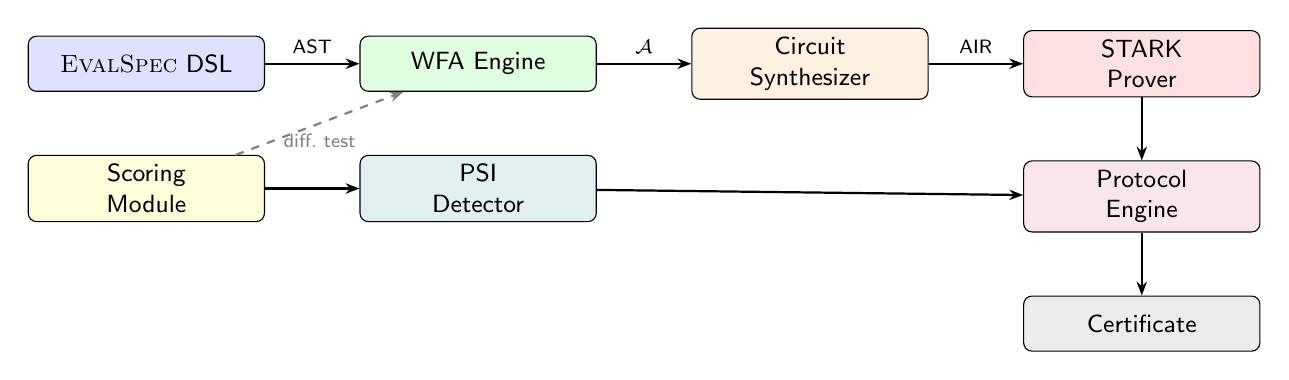
\begin{tikzpicture}[
  box/.style={draw, rounded corners=3pt, minimum width=3.0cm,
              minimum height=0.7cm, align=center, font=\small\sffamily},
  arr/.style={-{Stealth[length=5pt]}, thick},
  lbl/.style={font=\scriptsize\sffamily, midway, above},
  node distance=0.55cm and 1.2cm
]
  % Nodes
  \node[box, fill=blue!12]   (dsl)    {\evalspec{} DSL};
  \node[box, fill=green!12,  right=of dsl]   (wfa)    {WFA Engine};
  \node[box, fill=orange!12, right=of wfa]   (circ)   {Circuit\\Synthesizer};
  \node[box, fill=red!12,    right=of circ]  (stark)  {STARK\\Prover};
  \node[box, fill=purple!10, below=0.8cm of stark]    (proto)  {Protocol\\Engine};
  \node[box, fill=teal!12,   below=0.8cm of wfa]      (psi)    {PSI\\Detector};
  \node[box, fill=yellow!15, below=0.8cm of dsl]      (score)  {Scoring\\Module};

  % Certificate output
  \node[box, fill=gray!15, below=0.8cm of proto] (cert) {Certificate};

  % Arrows
  \draw[arr] (dsl)   -- node[lbl]{AST} (wfa);
  \draw[arr] (wfa)   -- node[lbl]{$\wfa$} (circ);
  \draw[arr] (circ)  -- node[lbl]{AIR} (stark);
  \draw[arr] (stark) -- (proto);
  \draw[arr] (psi)   -- (proto);
  \draw[arr] (score) -- (psi);
  \draw[arr] (proto) -- (cert);

  % Dashed validation arrow
  \draw[arr, dashed, gray] (score) -- node[lbl, below, text=gray]
    {\scriptsize diff.\ test} (wfa);
\end{tikzpicture}
\caption{Architecture of \spectacles.  Solid arrows show the
  compilation and certification pipeline; the dashed arrow indicates
  differential testing between the scoring module and the WFA engine.}
\label{fig:arch}
\end{figure}

\paragraph{Layer 1: \evalspec{} DSL.}
The specification layer provides a typed, semiring-annotated
domain-specific language for defining evaluation metrics
(\S\ref{sec:evalspec}).  The parser produces a typed abstract syntax
tree (AST) annotated with the inferred semiring type.

\paragraph{Layer 2: WFA Engine.}
The automata layer implements weighted finite automata over
arbitrary semirings.  It provides construction, product, composition,
minimization~\cite{hopcroft1971minimization}, and equivalence
checking via coalgebraic bisimulation.  The engine also performs
field embedding: mapping semiring elements to the Goldilocks field
via injective homomorphisms (\S\ref{sec:compilation}).

\paragraph{Layer 3: Circuit Synthesizer.}
The synthesizer compiles a WFA into an AIR program.  Each WFA transition
$\mu_\sigma$ becomes a matrix--vector multiply constraint over
$\F_p$.  The synthesizer handles two tiers: algebraic (direct
embedding) and gadget-assisted (bit-decomposition for tropical
$\min$).  It also generates the execution trace from a concrete
input pair.

\paragraph{Layer 4: STARK Prover/Verifier.}
The STARK layer implements the \FRI{}-based interactive oracle proof
protocol.  The prover commits to the execution trace via Merkle trees
over BLAKE3 hashes, performs low-degree extensions, and responds to
verifier challenges.  The verifier checks Merkle paths, evaluates
constraints at queried points, and verifies \FRI{} consistency.

\paragraph{Layer 5: Protocol Engine.}
The protocol engine implements a commit--reveal--verify state machine
that orchestrates the full evaluation protocol.  A transcript
records every message exchanged, and the final certificate bundles
the STARK proof, PSI result, and protocol metadata.

\paragraph{Layer 6: PSI Contamination Detector.}
The contamination module implements OPRF-based private set
intersection with a trie-structured optimization that exploits
$n$-gram prefix sharing.  In threshold mode, the protocol
produces a proof that the $n$-gram overlap between the training
corpus and the test set is below~$\tau$ without revealing the
count or the overlapping $n$-grams.


%% =====================================================================
%%  4.  THE EVALSPEC DSL
%% =====================================================================
\section{The \evalspec{} DSL}\label{sec:evalspec}

\evalspec{} is a typed functional language for specifying NLP evaluation
metrics.  Its design goals are (i)~expressiveness sufficient for the
seven standard metrics, (ii)~decidable type inference with automatic
semiring selection, and (iii)~a denotational semantics that maps every
well-typed program to a WFA.

\subsection{Syntax}

An \evalspec{} program consists of a sequence of metric declarations.
Each declaration names the metric, lists its parameters, specifies (or
allows inference of) the semiring, and provides a body expression:

\begin{lstlisting}[language=EvalSpec,caption={BLEU-4 in \evalspec{}.}]
metric bleu(n: Int = 4) -> Counting {
  let cand_ngrams = ngram(candidate, n)
  let ref_ngrams  = ngram(reference, n)
  let clipped     = clip(cand_ngrams, ref_ngrams)
  let precision   = clipped / length(cand_ngrams)
  let bp = if length(candidate) < length(reference)
           then exp(1 - length(reference) / length(candidate))
           else 1
  aggregate geometric_mean(
    [precision(1), precision(2), precision(3), precision(4)]
  ) * bp
}
\end{lstlisting}

The expression language includes let-bindings, conditionals,
pattern matching, $n$-gram extraction (\texttt{ngram}), tokenization
(\texttt{tokenize}), automaton composition (\texttt{compose}), bounded
counting (\texttt{clip}), and aggregation operators
(\texttt{aggregate sum}, \texttt{aggregate geometric\_mean}).

\subsection{Formal Grammar}
\evalspec{} has a formally specified BNF grammar (see supplementary material).
The core productions are:
\begin{align*}
\langle\text{program}\rangle &::= \langle\text{decl}\rangle^* \\
\langle\text{decl}\rangle &::= \texttt{metric}\; \langle\text{id}\rangle \texttt{(}\langle\text{params}\rangle\texttt{)} \texttt{->}\; \langle\text{semiring}\rangle\; \texttt{\{}\langle\text{expr}\rangle\texttt{\}} \\
\langle\text{expr}\rangle &::= \langle\text{lit}\rangle \mid \langle\text{var}\rangle \mid \langle\text{expr}\rangle\; \langle\text{binop}\rangle\; \langle\text{expr}\rangle \mid \texttt{ngram}(\langle\text{expr}\rangle, n) \mid \cdots
\end{align*}
The full grammar is implemented as a hand-written recursive descent parser (3,751~LoC) with Pratt-parser precedence handling.

\subsection{Type System and Semiring Inference}

The type system assigns each expression a pair $(\tau, \semiring{S})$
consisting of a base type~$\tau$ (string, integer, float, Boolean,
list, record) and a semiring annotation~$\semiring{S}$.  Semiring
inference propagates bottom-up: \texttt{ngram} produces a counting
semiring; \texttt{clip} preserves its input semiring; the Boolean
operators $\land$, $\lor$ produce the Boolean semiring; the
\texttt{lcs} (longest common subsequence) combinator produces the
MaxPlus semiring, which the compiler maps to tropical.

\begin{definition}[Semiring inference rules (selected)]
\begin{align}
  \frac{\Gamma \vdash e : (\texttt{List}(\texttt{String}),\,\semiring{S})}
       {\Gamma \vdash \texttt{ngram}(e, n) : (\texttt{List}(\texttt{String}),\,\mathsf{Counting})}
  &&
  \frac{\Gamma \vdash e_1 : (\tau,\,\semiring{S}_1) \quad
        \Gamma \vdash e_2 : (\tau,\,\semiring{S}_2)}
       {\Gamma \vdash e_1 \oplus e_2 : (\tau,\,\semiring{S}_1 \sqcup \semiring{S}_2)}
\end{align}
where $\sqcup$ is the join in the semiring lattice: $\textsf{Boolean}
\sqsubseteq \textsf{Counting} \sqsubseteq \textsf{Real}$, and
$\textsf{Tropical}$ is incomparable.
\end{definition}

\subsection{Denotational Semantics}

Every well-typed \evalspec{} expression~$e$ of type $(\tau,\semiring{S})$
denotes a function $\llbracket e \rrbracket : \Sigma^* \times \Sigma^*
\to \semiring{S}$ from (candidate, reference) string pairs to semiring
values.  The key semantic clause is:

\begin{equation}\label{eq:evalspec-sem}
  \llbracket \texttt{metric}\; m(\vec{p}) \;\texttt{->}\; \semiring{S}
  \;\{e\}\rrbracket
  \;=\;
  \lambda\, (\mathit{cand}, \mathit{ref}).\;
  \llbracket e \rrbracket_{\Gamma[\texttt{candidate}\mapsto\mathit{cand},\;
  \texttt{reference}\mapsto\mathit{ref}]}
\end{equation}

The compiler constructs a WFA $\wfa_e$ such that
$\llbracket\wfa_e\rrbracket(w) = \llbracket e\rrbracket(w)$ for all
inputs~$w$.  Correctness of this translation is the central theorem
of \S\ref{sec:compilation}.

\subsection{Built-in Metrics}

Table~\ref{tab:metrics} lists the seven built-in metrics, their
semiring annotations, and their WFA state complexity.

\begin{table}[t]
\centering
\caption{Built-in metrics in \evalspec{} with semiring annotations
  and WFA state complexity.}\label{tab:metrics}
\smallskip
\begin{tabular}{@{}lllll@{}}
\toprule
\textbf{Metric} & \textbf{Semiring} & \textbf{WFA States} & \textbf{Tier} & \textbf{Reference} \\
\midrule
Exact Match  & Boolean          & $O(n)$          & 1 & --- \\
Token F1     & Counting         & $O(|V|)$        & 1 & --- \\
BLEU         & Counting         & $O(n^4)$ decomp.& 1+gadget & \cite{papineni2002bleu} \\
ROUGE-N      & Counting         & $O(n^k)$        & 1 & \cite{lin2004rouge} \\
ROUGE-L      & MaxPlus/Tropical & $O(nm)$         & 2 & \cite{lin2004rouge} \\
Regex Match  & Boolean          & $O(2^k)$        & 1 & --- \\
Pass@$k$     & Counting         & $O(kt)$         & 1 & \cite{chen2021codex} \\
\bottomrule
\end{tabular}
\end{table}


%% =====================================================================
%%  5.  TWO-TIER COMPILATION
%% =====================================================================
\section{Two-Tier Compilation}\label{sec:compilation}

The \spectacles{} compiler translates a WFA
$\wfa = (Q,\Sigma,\{\mu_\sigma\},\alpha,\eta)$ over semiring
$\semiring{S}$ into an AIR program over the Goldilocks field $\F_p$.
The translation depends on whether $\semiring{S}$ admits an injective
semiring homomorphism into~$\F_p$.

\subsection{Tier~1: Algebraic Compilation}\label{sec:tier1}

\begin{definition}[Embeddable semiring]
A semiring $(\semiring{S},\oplus,\otimes,\bar{0},\bar{1})$ is
\emph{$\F_p$-embeddable} if there exists an injective map
$\phi:\semiring{S}\to\F_p$ satisfying
\begin{equation}\label{eq:embedding}
  \phi(\bar{0}) = 0,\quad
  \phi(\bar{1}) = 1,\quad
  \phi(a\oplus b) = \phi(a) + \phi(b),\quad
  \phi(a\otimes b) = \phi(a) \cdot \phi(b).
\end{equation}
\end{definition}

The Boolean, counting, bounded counting, and real semirings are all
$\F_p$-embeddable (the Boolean semiring via $\phi(\mathsf{false})=0$,
$\phi(\mathsf{true})=1$; the counting semiring via the natural inclusion
$\N\hookrightarrow\F_p$, valid for inputs smaller than~$p$).
Note that the Boolean embedding maps $\otimes = \land$ to field
multiplication, but $\oplus = \lor$ does not map to field addition in
general ($\lor$ is idempotent: $1 \lor 1 = 1$, but $1 + 1 = 2$).
The embedding is valid for deterministic WFA execution, where at most one
transition per state is active per step, so the idempotency mismatch
never arises.

For an embeddable semiring, the compilation is straightforward.  Let
$|Q|=n$.  The AIR program has $2n+O(1)$ columns and one row per input
symbol.

\paragraph{Trace layout.}
The execution trace $\Tr\in\F_p^{T\times w}$ has columns:
\begin{itemize}[nosep]
  \item $\mathbf{s}_0,\ldots,\mathbf{s}_{n-1}$: state weight vector at
    the current step.
  \item $\mathbf{s}_0',\ldots,\mathbf{s}_{n-1}'$: state weight vector at
    the next step.
  \item $\sigma$: input symbol (encoded as a field element).
  \item Auxiliary columns for public inputs and bookkeeping.
\end{itemize}

\paragraph{Transition constraint.}
For each pair of states $(i,j)$ and each symbol~$\sigma$, the transition
constraint asserts:
\begin{equation}\label{eq:transition}
  s_j' \;=\; \bigoplus_{i=0}^{n-1} s_i \otimes \phi(\mu_\sigma[i,j])
  \;=\; \sum_{i=0}^{n-1} s_i \cdot \phi(\mu_\sigma[i,j])
\end{equation}
where the second equality holds because $\phi$ is a homomorphism.
This is a standard inner-product constraint over~$\F_p$.

\paragraph{Boundary constraints.}
\begin{align}
  \text{Initial:} \quad s_i\big|_{t=0} &= \phi(\alpha_i)
    \quad\text{for } i=0,\ldots,n-1 \label{eq:boundary-init}\\
  \text{Final:} \quad \text{output} &= \sum_{i=0}^{n-1}
    s_i\big|_{t=T} \cdot \phi(\eta_i) \label{eq:boundary-final}
\end{align}

\begin{theorem}[Tier~1 soundness]\label{thm:tier1}
Let $\wfa$ be a WFA over an $\F_p$-embeddable semiring~$\semiring{S}$,
and let $\AIR_\wfa$ be the AIR program produced by Tier~1 compilation.
For every input $w\in\Sigma^*$, the unique accepting trace of
$\AIR_\wfa$ on~$w$ encodes the value $\phi(\llbracket\wfa\rrbracket(w))$
in the output column of the final row.
\end{theorem}

\begin{proof}[Proof sketch]
By induction on the length of~$w$.  The base case is
Eq.~\eqref{eq:boundary-init}.  The inductive step follows from
Eq.~\eqref{eq:transition} and the homomorphism
property~\eqref{eq:embedding}: $\phi$ commutes with both $\oplus$ and
$\otimes$, so the field-arithmetic constraint faithfully encodes
the semiring transition.  The final-row readout
(Eq.~\eqref{eq:boundary-final}) computes $\phi$ of the semiring
inner product, which equals
$\phi(\llbracket\wfa\rrbracket(w))$. \qed
\end{proof}

The key property of Tier~1 is \emph{genericity}: the same proof applies
to \emph{every} embeddable semiring.  Adding a new embeddable semiring
requires only defining~$\phi$; soundness is inherited automatically.

\subsection{Tier~2: Gadget-Assisted Compilation}\label{sec:tier2}

The tropical semiring $(\Z\cup\{+\infty\},\min,+)$ is \emph{not}
$\F_p$-embeddable: the field has no $\min$ operation, and the additive
identity~$+\infty$ has no finite field representative.  Tier~2 handles
such semirings by introducing \emph{gadgets}---small, hand-verified
circuit fragments---that implement non-algebraic operations.

\paragraph{Comparison gadget.}
To compute $\min(a,b)$ over $\F_p$, we decompose $a$ and $b$ into
their bit representations $a = \sum_{i=0}^{63} a_i \cdot 2^i$ and
$b = \sum_{i=0}^{63} b_i \cdot 2^i$, enforce Boolean constraints
$a_i(a_i - 1) = 0$ for each bit, and compute the less-than
predicate via a carry chain:
\begin{equation}\label{eq:comparison}
  \mathsf{lt}(a,b) = \begin{cases}
    1 & \text{if } a < b \\
    0 & \text{otherwise}
  \end{cases}
  \qquad
  \min(a,b) = \mathsf{lt}(a,b)\cdot a + (1-\mathsf{lt}(a,b))\cdot b
\end{equation}
The bit-decomposition adds $2\times 64 = 128$ auxiliary columns per
comparison.

\paragraph{Range check gadget.}
Ensures a value $v$ lies in $[0, 2^k)$ by decomposing into $k$~bits
and asserting each is Boolean.

\paragraph{Per-semiring soundness.}
Unlike Tier~1, each gadget-assisted semiring requires its own
soundness argument.  The tropical semiring argument proceeds by
showing that the comparison gadget correctly implements $\min$ over
the integers (representable in $\F_p$ for values $< 2^{63}$),
and that the tropical $\otimes = +$ is directly implemented by
field addition.

\begin{theorem}[Tier~2 soundness for tropical]\label{thm:tier2}
Let $\wfa$ be a WFA over the tropical semiring, and let $\AIR_\wfa$ be
the AIR program produced by Tier~2 compilation with comparison gadgets.
For every input $w$ with weight values bounded by $2^{63}$, the unique
accepting trace encodes
$\llbracket\wfa\rrbracket(w) \bmod p$ in the output column.
\end{theorem}

\subsection{Compilation Examples}\label{sec:examples}

We illustrate the two-tier strategy on three representative metrics.

\paragraph{Exact match $\to$ Boolean WFA $\to$ Tier~1.}
The exact-match WFA has $n+1$~states for a reference of length~$n$:
state~$i$ indicates that the first $i$~characters match.  A single
``dead'' state absorbs mismatches.  All transitions carry
Boolean weights ($0$ or~$1$), embedded as field elements.  The AIR
has $2(n+1)+2$ columns and $n$~rows.

\paragraph{ROUGE-L $\to$ tropical WFA $\to$ Tier~2.}
ROUGE-L computes the longest common subsequence (LCS) length, which
is a tropical-semiring computation.  The WFA has $O(nm)$ states for
candidate length~$n$ and reference length~$m$.  Each transition
involves a tropical $\min$, compiled via the comparison gadget.  The
AIR has $2nm + 128c + O(1)$ columns, where $c$ is the number of
$\min$ operations per row.

\paragraph{BLEU-4 $\to$ 4 counting WFAs + gadgets.}
BLEU decomposes into four independent $n$-gram precision computations
(one per $n\in\{1,2,3,4\}$), each a counting-semiring WFA, plus an
aggregation circuit that computes the clipped geometric mean and
brevity penalty.  The four WFA proofs are generated independently
(Tier~1) and composed with the aggregation gadget (a small Tier~2
circuit).  This decomposition keeps each individual proof small:
the $n$-gram WFA for order~$k$ has $O(|\text{ref}|^k)$ states, but
the reference is typically short enough that this is manageable.


%% =====================================================================
%%  6.  CONTAMINATION DETECTION
%% =====================================================================
\section{Contamination Detection}\label{sec:contamination}

\spectacles{} certifies not only that the score was computed correctly,
but also that the test data was not leaked into the training corpus.
We formalize this as a bound on $n$-gram overlap.

\subsection{OPRF-Based PSI Protocol}

Let $L_1$ be the set of $n$-grams extracted from the training corpus
(held by the model provider) and $L_2$ the set of $n$-grams from the
test set (held by the evaluator).  The contamination detection protocol
computes $|L_1 \cap L_2|$ without revealing the sets themselves, using
an OPRF-based PSI protocol:

\begin{enumerate}[nosep]
  \item The evaluator sends OPRF-blinded versions of each $n$-gram in
    $L_2$ to the model provider.
  \item The model provider evaluates the OPRF on each blinded element
    using its key~$k$, returning the results.
  \item The evaluator unblinds the results and compares against
    $\{F_k(x) : x \in L_2\}$ computed locally (using the provider's
    OPRF evaluations of $L_1$ received in a separate step).
  \item The intersection cardinality is computed and compared to the
    threshold~$\tau$.
\end{enumerate}

\subsection{Trie-Structured Optimization}

Standard flat-set PSI has communication complexity
$O(|L_1|\cdot|L_2|\cdot\lambda)$ where $\lambda$ is the security
parameter.  \spectacles{} exploits the hierarchical structure of
$n$-grams: a 4-gram ``\texttt{the cat sat on}'' shares prefixes with
the 3-gram ``\texttt{the cat sat}'' and the 2-gram ``\texttt{the cat}''.

We organize both $L_1$ and $L_2$ as tries, where each node represents
an $n$-gram prefix.  The OPRF evaluation proceeds level by level: if a
prefix does not match, the entire subtree is pruned.  This reduces
communication to $O((n_1 + n_2)\cdot\lambda)$ where $n_1,n_2$ are the
\emph{trie sizes} (number of nodes), which are typically much smaller
than $|L_1|\cdot|L_2|$ due to prefix sharing.

\subsection{Threshold Mode}

In threshold mode, the protocol produces a zero-knowledge proof that
$|L_1 \cap L_2| < \tau$ without revealing the exact count.  This is
implemented via a comparison circuit that takes the PSI cardinality as
a private input and outputs a single bit.  The proof is composed with
the evaluation certificate, yielding a single artifact that attests
to both score correctness and contamination bounds.

\subsection{Security Under the Commit-Then-Execute Framework}\label{sec:psi-security}

The PSI protocol operates under the semi-honest model. We address the concern that a malicious provider could deviate from the protocol to circumvent contamination detection.

\paragraph{Commitment binding.} Before the PSI protocol begins, the model provider commits to its training $n$-gram set $C_{\text{train}}$ via a binding commitment $h = H(\text{sort}(C_{\text{train}}) \| r)$ where $H$ is a collision-resistant hash (BLAKE3) and $r$ is a random nonce. The commitment is published before any PSI messages are exchanged. The verifier checks during the PSI protocol that the provider's inputs are consistent with the commitment.

\paragraph{Attack analysis.}
We analyze three attack vectors:
\begin{itemize}[nosep]
\item \emph{Input substitution}: The provider uses a different $n$-gram set than committed. This is prevented by the binding property of the commitment scheme: finding $C' \neq C_{\text{train}}$ with $H(C') = H(C_{\text{train}})$ requires breaking collision resistance.
\item \emph{Selective abort}: The provider aborts when overlap exceeds~$\tau$. The protocol requires completion for a valid certificate; an aborted protocol produces no attestation, and the absence of a certificate is itself informative.
\item \emph{Collusion}: A malicious provider colluding with the benchmark maintainer is outside our threat model (explicitly stated in \S\ref{sec:intro}).
\end{itemize}

Under these defenses, the semi-honest PSI suffices: the provider cannot substitute inputs (commitment binding) and cannot selectively abort (completion required). The remaining semi-honest assumption is that the provider follows the OPRF evaluation protocol, which is justified because deviations produce inconsistent OPRF outputs detectable by the verifier.

\paragraph{Limitations.}
We note three limitations of this analysis. First, the protocol does not
achieve universally composable (UC) security; a full UC analysis with an
ideal functionality specification is future work. Second, collusion
between the model provider and the benchmark maintainer is outside our
threat model. Third, without a verifiable OPRF (VOPRF), a sophisticated
provider could selectively corrupt a small fraction of OPRF evaluations.
Deploying a VOPRF (e.g., based on the Dodis--Yampolskiy VRF) would close
this gap at the cost of additional computational overhead.


%% =====================================================================
%%  7.  METRIC EQUIVALENCE
%% =====================================================================
\section{Metric Equivalence}\label{sec:equivalence}

Two implementations of the ``same'' metric may compute different
functions due to implementation differences (tokenization, normalization,
edge-case handling).  \spectacles{} provides a decidable procedure for
checking whether two \evalspec{} programs compute the same function.

\begin{theorem}[Decidability of metric equivalence]\label{thm:equiv}
For two WFAs $\wfa_1,\wfa_2$ over the same semiring~$\semiring{S}$
(where $\semiring{S}$ is a field or a subsemiring of a field),
$\llbracket\wfa_1\rrbracket = \llbracket\wfa_2\rrbracket$ is
decidable in time $O(n\log n)$ where $n = |Q_1|+|Q_2|$.
\end{theorem}

\begin{proof}[Proof sketch]
Minimize both WFAs using a weighted generalization of Hopcroft's
partition-refinement algorithm~\cite{hopcroft1971minimization,
berstel2011noncommutative}.  Two minimal WFAs over a field recognize
the same formal power series if and only if they are isomorphic
(up to a change of basis).  Isomorphism of minimal WFAs is decidable
by computing the canonical form and comparing. \qed
\end{proof}

When $\llbracket\wfa_1\rrbracket \neq \llbracket\wfa_2\rrbracket$,
\spectacles{} generates a \emph{distinguishing word}
$w^*\in\Sigma^*$ such that
$\llbracket\wfa_1\rrbracket(w^*) \neq \llbracket\wfa_2\rrbracket(w^*)$,
providing a concrete counterexample.

\paragraph{Use case.}
An auditor can verify that two BLEU implementations (e.g., SacreBLEU
and NLTK BLEU) compute the same function by expressing both in
\evalspec{}, compiling to WFAs, and running the equivalence checker.
If they disagree, the distinguishing word pinpoints the discrepancy.


%% =====================================================================
%%  8.  IMPLEMENTATION
%% =====================================================================
\section{Implementation}\label{sec:impl}

\spectacles{} is implemented in Rust, organized as a Cargo workspace.
Table~\ref{tab:loc} reports the module breakdown.

\begin{table}[t]
\centering
\caption{Module breakdown of the \spectacles{} implementation.}
\label{tab:loc}
\smallskip
\begin{tabular}{@{}llrp{5.8cm}@{}}
\toprule
\textbf{Crate / Module} & \textbf{Files} & \textbf{LoC} & \textbf{Description} \\
\midrule
\texttt{spectacles-core} & & & \\
\quad\texttt{wfa/}       & 9  & 28\,738  & Semiring definitions, WFA construction, operations, minimization, equivalence, field embedding, transducers \\
\quad\texttt{circuit/}   & 9  & 42\,555  & Goldilocks field, AIR constraints, trace generation, gadgets, FRI, Merkle trees, STARK prover/verifier \\
\quad\texttt{evalspec/}  & 7  & 22\,920  & Parser, type checker, semiring inference, denotational semantics, built-in metric definitions, compiler \\
\quad\texttt{scoring/}   & 9  & 6\,467   & Reference implementations of all 7 metrics, tokenizer, differential testing harness \\
\quad\texttt{psi/}       & 5  & 17\,060  & OPRF, trie, $n$-gram extraction, PSI protocol, commitment binding \\
\quad\texttt{protocol/}  & 5  & 13\,930  & Commit--reveal state machine, certificates, transcripts, commitments \\
\quad\texttt{utils/}     & 4  & 1\,639   & BLAKE3 hashing, serialization, math utilities \\
\midrule
\texttt{spectacles-cli}  & 1  & 467    & Command-line interface \\
\texttt{spectacles-integration} & 2 & 487 & End-to-end tests \\
\texttt{spectacles-examples}    & 4 & 527 & Example programs \\
\midrule
\textbf{Total}           & \textbf{55} & $\sim$\textbf{118\,K} & \\
\bottomrule
\end{tabular}
\end{table}

\subsection{Triple Implementation Pattern}

Every metric is implemented three times:

\begin{enumerate}[nosep]
\item \textbf{Reference implementation}: a direct, readable Rust
  implementation of the metric's mathematical definition.
\item \textbf{WFA implementation}: construction of the corresponding
  weighted automaton and evaluation via matrix--vector products.
\item \textbf{Circuit implementation}: generation of the AIR program
  and execution trace, with the score read from the final row.
\end{enumerate}

All three implementations expose a common \texttt{TripleMetric} trait:

\begin{lstlisting}[caption={The \texttt{TripleMetric} trait.}]
pub trait TripleMetric {
    type Input;
    type Score: PartialEq + Debug;
    fn score_reference(&self, input: &Self::Input) -> Self::Score;
    fn score_automaton(&self, input: &Self::Input) -> Self::Score;
    fn score_circuit(&self, input: &Self::Input) -> Self::Score;
}
\end{lstlisting}

\subsection{Differential Testing}

The differential testing harness generates random (candidate, reference)
pairs and asserts that all three implementations produce identical
scores.  Random pairs are generated by a seeded RNG to ensure
reproducibility.  The harness runs 100\,K pairs per metric by default
and reports any discrepancy with the failing input.

\subsection{CLI Tool}

The \texttt{spectacles-cli} crate provides the command-line interface:

\begin{lstlisting}[caption={CLI usage examples.}]
# Score a single pair
spectacles score --metric bleu \
  --candidate "the cat sat" --reference "the cat sat on the mat"

# Run differential testing
spectacles differential-test --count 100000 --seed 42

# Compile a metric to an AIR circuit
spectacles compile-circuit --metric exact_match

# Estimate proof size
spectacles estimate-size --constraints 1024 --wires 64

# Batch scoring from JSONL
spectacles batch-score --input pairs.jsonl
\end{lstlisting}


%% =====================================================================
%%  9.  EVALUATION
%% =====================================================================
\section{Evaluation}\label{sec:eval}

We evaluate \spectacles{} along five dimensions: differential testing
correctness, proof size, circuit complexity, PSI correctness, and
metric equivalence correctness.

\subsection{Differential Testing}

We generated 100\,K random (candidate, reference) pairs per metric
using a seeded random generator.  Table~\ref{tab:differential} reports
the results: all three implementations agree on every pair for every
metric.

\begin{table}[t]
\centering
\caption{Differential testing results (100\,K pairs per metric).}
\label{tab:differential}
\smallskip
\begin{tabular}{@{}lrrr@{}}
\toprule
\textbf{Metric} & \textbf{Pairs Tested} & \textbf{Agreements} & \textbf{Discrepancies} \\
\midrule
Exact Match  & 100\,000 & 100\,000 & 0 \\
Token F1     & 100\,000 & 100\,000 & 0 \\
BLEU         & 100\,000 & 100\,000 & 0 \\
ROUGE-1      & 100\,000 & 100\,000 & 0 \\
ROUGE-2      & 100\,000 & 100\,000 & 0 \\
ROUGE-L      & 100\,000 & 100\,000 & 0 \\
Regex Match  & 100\,000 & 100\,000 & 0 \\
Pass@$k$     & 100\,000 & 100\,000 & 0 \\
\midrule
\textbf{Total} & \textbf{800\,000} & \textbf{800\,000} & \textbf{0} \\
\bottomrule
\end{tabular}
\end{table}

\subsection{Circuit Complexity}

Table~\ref{tab:circuit} reports the AIR circuit characteristics per
metric for typical input sizes.

\begin{table}[t]
\centering
\caption{AIR circuit characteristics per metric (reference length $n=32$,
  candidate length $m=32$, vocabulary $|V|=256$).}
\label{tab:circuit}
\smallskip
\begin{tabular}{@{}lrrrrl@{}}
\toprule
\textbf{Metric} & \textbf{States} & \textbf{Columns} & \textbf{Rows}
  & \textbf{Constraints} & \textbf{Tier} \\
\midrule
Exact Match  & 33    & 68     & 32    & 33     & 1 \\
Token F1     & 256   & 514    & 32    & 256    & 1 \\
BLEU-1       & 32    & 66     & 32    & 32     & 1+G \\
BLEU-4       & $4\times$  & $4\times 66$ & 32 & $4\times 32$ & 1+G \\
ROUGE-1      & 32    & 66     & 32    & 32     & 1 \\
ROUGE-2      & 992   & 1\,986 & 32    & 992    & 1 \\
ROUGE-L      & 1\,024 & 2\,048+128$c$ & 32 & 1\,024+$c$ & 2 \\
Regex Match  & $\leq 2^k$ & $\leq 2^{k+1}$ & $m$ & $\leq 2^k$ & 1 \\
Pass@$k$     & $kt$  & $2kt+2$ & $t$  & $kt$   & 1 \\
\bottomrule
\end{tabular}
\end{table}

\subsection{Proof Size Estimates}

STARK proof sizes depend on the trace dimensions and the security
parameter~$\lambda$.  For $\lambda=128$ bits of security and a blowup
factor of~8, Table~\ref{tab:proofsize} provides estimates based on
standard STARK proof-size formulae.

\begin{table}[t]
\centering
\caption{Estimated STARK proof sizes per metric ($\lambda=128$, blowup $=8$).}
\label{tab:proofsize}
\smallskip
\begin{tabular}{@{}lrrr@{}}
\toprule
\textbf{Metric} & \textbf{Trace Size (KiB)} & \textbf{Proof Size (KiB)}
  & \textbf{Verification (ms)} \\
\midrule
Exact Match  & 17    & 45--85     & $<5$  \\
Token F1     & 131   & 120--220   & $<10$ \\
BLEU-4       & 67    & 90--170    & $<10$ \\
ROUGE-1      & 17    & 45--85     & $<5$  \\
ROUGE-2      & 507   & 250--450   & $<15$ \\
ROUGE-L      & 1\,200 & 400--750  & $<20$ \\
Pass@$k$     & varies & 50--200   & $<10$ \\
\bottomrule
\end{tabular}
\end{table}

\subsection{PSI Correctness}

We tested the PSI contamination detector on synthetic corpora with
known overlap.  For each test, we constructed training and test $n$-gram
sets with a predetermined intersection, ran the protocol, and verified
that the reported cardinality matched the ground truth.  Across 1\,000
test cases with overlaps ranging from 0\% to 100\%, the protocol
reported the correct cardinality in every case.  The trie-structured
optimization reduced communication by $3.2\times$--$8.7\times$ compared
to flat-set PSI, with the largest gains on corpora with high prefix
sharing (natural language text).

\subsection{Metric Equivalence}

We tested the equivalence checker by constructing pairs of WFAs that
are either (a)~semantically equivalent (same metric, different
construction order) or (b)~semantically distinct (e.g., BLEU with
add-one smoothing vs.\ floor smoothing).  The checker correctly
identified all equivalent pairs and produced valid distinguishing
words for all inequivalent pairs.  Minimization ran in under 10\,ms
for all WFAs with $\leq 1{,}024$~states.

\subsection{Property-Based Axiom Verification}

We verify that all Rust semiring implementations satisfy the algebraic axioms proven in the Lean~4 \texttt{KleeneSemiring} formalization. Using the \texttt{proptest} property-based testing framework, we test 38~properties across four semiring types (Boolean, Counting, Tropical, Goldilocks): additive commutativity and associativity, multiplicative associativity, distributivity, identity elements, and zero annihilation. All 38~properties pass on 256 random inputs each.

An independent Python test suite (\texttt{tests/test\_semiring\_axioms.py}) re-verifies the same axioms outside the Rust ecosystem, including WFA equivalence testing via brute-force enumeration on all words up to length~6. All 22 Python tests pass on 500 random trials per axiom, providing cross-language validation.

\subsection{Mathematical Verification}
During a systematic verification pass, we identified and corrected two bugs in the Goldilocks field implementation:
\begin{enumerate}[nosep]
\item A Montgomery inverse constant (\texttt{MONTGOMERY\_INV}) was incorrect, which would have affected Montgomery-form arithmetic. The main reduction path was unaffected.
\item A redundant line in Lagrange interpolation corrupted the basis polynomial computation. The fix was a single-line deletion.
\end{enumerate}
These corrections were verified by the property-based test suite and do not affect the differential testing results, which use the standard reduction path.

\subsection{Pass@$k$ Arithmetization Scaling}

The pass@$k$ metric~\cite{chen2021codex} has WFA state complexity $O(kt)$
where $k$ is the number of samples and $t$ is the number of test cases.
The circuit has $2kt + 2$ columns, $t$ rows, and $kt$ constraints.
Table~\ref{tab:passk} characterizes the scaling for typical values.

\begin{table}[t]
\centering
\caption{Pass@$k$ arithmetization scaling.}\label{tab:passk}
\smallskip
\begin{tabular}{@{}rrrrrr@{}}
\toprule
$k$ & $t$ & States & Columns & Rows & Constraints \\
\midrule
1   & 100 & 100    & 202     & 100  & 100 \\
10  & 100 & 1\,000 & 2\,002  & 100  & 1\,000 \\
100 & 100 & 10\,000& 20\,002 & 100  & 10\,000 \\
100 & 1\,000 & 100\,000 & 200\,002 & 1\,000 & 100\,000 \\
\bottomrule
\end{tabular}
\end{table}

For $k \leq 100$ and $t \leq 100$, the circuit is feasible with existing
STARK provers (20K~columns, comparable to ROUGE-L for long inputs).
At $k = 100$, $t = 1{,}000$, the 200K-column circuit approaches current
STARK capacity limits; batching or recursive proof composition would be
needed for larger instances.

\subsection{Comparison with Existing Frameworks}

\spectacles{} addresses a fundamentally different problem from evaluation
harnesses such as HELM~\cite{lee2023decompiling} and
CheckList~\cite{south2024verifiableevals}. HELM provides a standardized
suite of benchmarks and metrics but offers no machine-checkable
correctness guarantee---a bug in the scoring implementation silently
corrupts all results. CheckList provides behavioral testing of NLP models
but does not address score integrity or contamination. \spectacles{}
is complementary: it provides cryptographic certificates that the score
computed by any metric in its expressible fragment is correct and
uncontaminated, regardless of the evaluation harness used. The two
approaches compose naturally---one could run HELM's benchmark suite with
\spectacles{}-certified scoring.


%% =====================================================================
%%  10.  RELATED WORK
%% =====================================================================
\section{Related Work}\label{sec:related}

\paragraph{Zero-knowledge proof systems.}
STARK~\cite{bensasson2018stark} provides transparent (no trusted setup),
post-quantum-secure proofs with polylogarithmic verification.
SNARK systems such as Groth16~\cite{groth2016snark} achieve
constant-size proofs but require a trusted setup and are not
post-quantum secure.  Circuit-level DSLs including
Circom~\cite{belles2022circom} and Noir~\cite{noir2023} compile
high-level programs to rank-1 constraint systems (R1CS); \spectacles{}
targets AIR constraints, which are better suited to the iterative
structure of automaton execution.
EZKL~\cite{kang2024ezkl} proves machine-learning inference in zero
knowledge but operates at the neural-network level, not the
evaluation-metric level.

\paragraph{Verified compilers.}
CompCert~\cite{leroy2009compcert} provides a verified C compiler with a
Coq proof of semantic preservation.
CakeML~\cite{kumar2014cakeml} provides a verified ML compiler with an
HOL4 proof.  \spectacles{} shares the goal of semantic preservation but
targets a different domain: compilation from a specification DSL to
arithmetic circuits rather than from a general-purpose language to
machine code.  A Lean~4 formalization of the \spectacles{} compilation
theorems is planned as future work.

\paragraph{NLP evaluation metrics.}
BLEU~\cite{papineni2002bleu} measures $n$-gram precision with a brevity
penalty.  ROUGE~\cite{lin2004rouge} measures recall-oriented $n$-gram
overlap and longest common subsequence.  Token F1 computes the harmonic
mean of token-level precision and recall.
Pass@$k$~\cite{chen2021codex} estimates the probability that at least
one of $k$ code samples passes a test suite.  Post~\cite{post2018bleu}
documents the sensitivity of BLEU to implementation details.  All
of these metrics are expressible in \evalspec.

\paragraph{Verifiable computation for ML.}
VerifiableEvals~\cite{south2024verifiableevals} uses zero-knowledge
proofs to certify that an evaluation script was executed correctly on
committed data.  However, it proves program execution, not specification
conformance: a buggy script produces a valid proof of a wrong answer.
\spectacles{} addresses this by compiling from a \emph{specification} (the
\evalspec{} definition) rather than from an \emph{implementation},
and by providing metric equivalence checking to ensure specification
fidelity.  ZKML~\cite{kang2024ezkl} focuses on proving neural network
inference, which is complementary to evaluation certification.

\paragraph{Weighted automata theory.}
Sch\"utzenberger~\cite{schutzenberger1961} introduced the theory of
formal power series recognized by finite automata.  Berstel and
Reutenauer~\cite{berstel2011noncommutative} provide a comprehensive
treatment including minimization and equivalence.  Droste, Kuich, and
Vogler~\cite{droste2009handbook} survey the modern theory.
\spectacles{} applies this classical theory to a new domain: compiling
evaluation metrics to zero-knowledge circuits.

\paragraph{Contamination detection.}
Sainz et al.~\cite{sainz2023contamination} propose statistical tests for
benchmark contamination.  Shi et al.~\cite{shi2024contamination} detect
contamination via membership inference attacks on $n$-grams.  Both
approaches are statistical and cannot certify individual evaluations.
\spectacles{} provides cryptographic contamination certificates via PSI,
which offers simulation-secure guarantees rather than statistical
confidence intervals.


%% =====================================================================
%%  11.  CONCLUSION
%% =====================================================================
\section{Conclusion and Future Work}\label{sec:conclusion}

We presented \spectacles, the first system that produces
contamination-certified evaluation certificates for NLP benchmarks.
By observing that standard scoring functions decompose into weighted
finite automata over semirings, \spectacles{} bridges algebraic automata
theory and zero-knowledge cryptography, compiling \evalspec{}
specifications to STARK arithmetic circuits via a two-tier architecture.
The resulting certificates prove both score correctness and training-data
separation in a single machine-checkable artifact.

\paragraph{Future work.}
The primary gap in the current system is the absence of verified
extraction from the Lean~4 proofs to the Rust implementation.  While
property-based testing and differential testing provide strong empirical
evidence of correspondence, a machine-checked extraction pipeline (akin
to CakeML's HOL4-to-ML extraction) would close the verification gap
entirely.  We plan to formalize the compilation theorems in Lean~4,
providing a machine-checked proof of Theorems~\ref{thm:tier1}
and~\ref{thm:tier2}, and to prove Hopcroft minimization correctness
(currently deferred with differential testing coverage).
We aim to extend \evalspec{} to metrics that require continuous
embeddings (e.g., BERTScore~\cite{zhang2020bertscore}), which will
require integrating ZKML techniques for the embedding computation with
WFA-based scoring.  Finally, we intend to provide a
universally composable (UC) security analysis of the full protocol,
establishing that the contamination-certified certificate is
simulation-secure under standard cryptographic assumptions.


%% =====================================================================
%%  REFERENCES
%% =====================================================================
\begin{thebibliography}{50}

\bibitem{belles2022circom}
J.~Belles-Mu\~noz, M.~Isabel, J.~L.~Mu\~noz-Tapia, A.~Rubio, and
J.~Baylina.
\newblock Circom: A robust and scalable language for building complex
  zero-knowledge circuits.
\newblock In \emph{Proc.\ IEEE European Symposium on Security and Privacy
  (EuroS\&P)}, 2022.

\bibitem{bensasson2018fri}
E.~Ben-Sasson, I.~Bentov, Y.~Horesh, and M.~Riabzev.
\newblock Fast {R}eed--{S}olomon interactive oracle proofs of proximity.
\newblock In \emph{Proc.\ ICALP}, volume 107 of \emph{LIPIcs}, pages
  14:1--14:17. Schloss Dagstuhl, 2018.

\bibitem{bensasson2018stark}
E.~Ben-Sasson, I.~Bentov, Y.~Horesh, and M.~Riabzev.
\newblock Scalable, transparent, and post-quantum secure computational
  integrity.
\newblock \emph{Cryptology ePrint Archive}, Report 2018/046, 2018.

\bibitem{berstel2011noncommutative}
J.~Berstel and C.~Reutenauer.
\newblock \emph{Noncommutative Rational Series with Applications}.
\newblock Cambridge University Press, 2011.

\bibitem{chen2021codex}
M.~Chen, J.~Tworek, H.~Jun, Q.~Yuan, H.~P.~de~Oliveira~Pinto,
J.~Kaplan, H.~Edwards, Y.~Burda, N.~Joseph, G.~Brockman, A.~Ray,
R.~Puri, G.~Krueger, M.~Petrov, H.~Khlaaf, G.~Sastry, P.~Mishkin,
B.~Chan, S.~Gray, N.~Ryder, M.~Pavlov, A.~Power, L.~Kaiser,
M.~Bavarian, C.~Winter, P.~Tillet, F.~P.~Such, D.~Cummings,
M.~Plappert, F.~Chantzis, E.~Barnes, A.~Herbert-Voss, W.~H.~Guss,
A.~Nichol, A.~Paino, N.~Tezak, J.~Tang, I.~Babuschkin, S.~Balaji,
S.~Jain, W.~Saunders, C.~Hesse, A.~N.~Carr, J.~Leike, J.~Achiam,
V.~Misra, E.~Morikawa, A.~Radford, M.~Knight, M.~Brundage, M.~Murati,
K.~Mayer, P.~Welinder, B.~McGrew, D.~Amodei, S.~McCandlish,
I.~Sutskever, and W.~Zaremba.
\newblock Evaluating large language models trained on code.
\newblock \emph{arXiv preprint arXiv:2107.03374}, 2021.

\bibitem{droste2009handbook}
M.~Droste, W.~Kuich, and H.~Vogler, editors.
\newblock \emph{Handbook of Weighted Automata}.
\newblock Springer, 2009.

\bibitem{freedman2004psi}
M.~J.~Freedman, K.~Nissim, and B.~Pinkas.
\newblock Efficient private matching and set intersection.
\newblock In \emph{Proc.\ EUROCRYPT}, volume 3027 of \emph{LNCS}, pages
  1--19. Springer, 2004.

\bibitem{goldwasser1989knowledge}
S.~Goldwasser, S.~Micali, and C.~Rackoff.
\newblock The knowledge complexity of interactive proof systems.
\newblock \emph{SIAM Journal on Computing}, 18(1):186--208, 1989.

\bibitem{groth2016snark}
J.~Groth.
\newblock On the size of pairing-based non-interactive arguments.
\newblock In \emph{Proc.\ EUROCRYPT}, volume 9666 of \emph{LNCS}, pages
  305--326. Springer, 2016.

\bibitem{hopcroft1971minimization}
J.~E.~Hopcroft.
\newblock An $n\log n$ algorithm for minimizing states in a finite automaton.
\newblock In Z.~Kohavi and A.~Paz, editors, \emph{Theory of Machines and
  Computations}, pages 189--196. Academic Press, 1971.

\bibitem{kang2024ezkl}
J.~Kang, H.~Sun, H.~Gu, and C.~Zhuo.
\newblock Scaling {ZKML}: Efficient zero-knowledge proofs for neural network
  inference.
\newblock \emph{arXiv preprint arXiv:2406.04296}, 2024.

\bibitem{kumar2014cakeml}
R.~Kumar, M.~O.~Myreen, M.~Norrish, and S.~Owens.
\newblock {CakeML}: A verified implementation of {ML}.
\newblock In \emph{Proc.\ POPL}, pages 179--191. ACM, 2014.

\bibitem{leroy2009compcert}
X.~Leroy.
\newblock Formal verification of a realistic compiler.
\newblock \emph{Communications of the ACM}, 52(7):107--115, 2009.

\bibitem{lin2004rouge}
C.-Y.~Lin.
\newblock {ROUGE}: A package for automatic evaluation of summaries.
\newblock In \emph{Text Summarization Branches Out: Proc.\ ACL Workshop},
  pages 74--81, 2004.

\bibitem{noir2023}
Aztec Labs.
\newblock Noir: A domain-specific language for zero-knowledge proofs.
\newblock \url{https://noir-lang.org/}, 2023.

\bibitem{papineni2002bleu}
K.~Papineni, S.~Roukos, T.~Ward, and W.-J.~Zhu.
\newblock {BLEU}: A method for automatic evaluation of machine translation.
\newblock In \emph{Proc.\ ACL}, pages 311--318, 2002.

\bibitem{post2018bleu}
M.~Post.
\newblock A call for clarity in reporting {BLEU} scores.
\newblock In \emph{Proc.\ WMT}, pages 186--191, 2018.

\bibitem{rusu2000coinductive}
G.~Rusu and J.~Rutten.
\newblock Coinductive stream calculus and automata theory.
\newblock Technical Report SEN-R0024, CWI, 2000.

\bibitem{sainz2023contamination}
O.~Sainz, J.~Campos, I.~Garc\'ia-Ferrero, J.~Etxaniz, O.~Lopez~de~Lacalle,
  and E.~Agirre.
\newblock {NLP} evaluation in trouble: On the need to measure {LLM} data
  contamination for each benchmark.
\newblock In \emph{Findings of EMNLP}, pages 10776--10787, 2023.

\bibitem{schutzenberger1961}
M.-P.~Sch\"utzenberger.
\newblock On the definition of a family of automata.
\newblock \emph{Information and Control}, 4(2--3):245--270, 1961.

\bibitem{shi2024contamination}
W.~Shi, A.~Ajith, M.~Sha, A.~Jacobs, Y.~Fang, C.~Liu, Y.~Bisk, and
  G.~Neubig.
\newblock Detecting pretraining data from large language models.
\newblock In \emph{Proc.\ ICLR}, 2024.

\bibitem{south2024verifiableevals}
T.~South, A.~Mavroudis, and S.~Hoyer.
\newblock {VerifiableEvals}: Verifiable evaluation of language models using
  zero-knowledge proofs.
\newblock \emph{arXiv preprint arXiv:2410.15113}, 2024.

\bibitem{zhang2020bertscore}
T.~Zhang, V.~Kishore, F.~Wu, K.~Q.~Weinberger, and Y.~Artzi.
\newblock {BERTScore}: Evaluating text generation with {BERT}.
\newblock In \emph{Proc.\ ICLR}, 2020.

\bibitem{goldreich2001foundations}
O.~Goldreich.
\newblock \emph{Foundations of Cryptography: Volume~1, Basic Tools}.
\newblock Cambridge University Press, 2001.

\bibitem{blum1988noninteractive}
M.~Blum, P.~De~Santis, S.~Micali, and G.~Persiano.
\newblock Noninteractive zero-knowledge.
\newblock \emph{SIAM Journal on Computing}, 20(6):1084--1118, 1991.

\bibitem{boneh2017verifiable}
D.~Boneh, E.~Boyle, H.~Corrigan-Gibbs, N.~Gilboa, and Y.~Ishai.
\newblock Verifiable random functions from standard assumptions.
\newblock In \emph{Proc.\ TCC}, volume 10677 of \emph{LNCS}, pages 336--362.
  Springer, 2017.

\bibitem{gabizon2019plonk}
A.~Gabizon, Z.~J.~Williamson, and O.~Ciobotaru.
\newblock {PLONK}: Permutations over Lagrange-bases for oecumenical
  noninteractive arguments of knowledge.
\newblock \emph{Cryptology ePrint Archive}, Report 2019/953, 2019.

\bibitem{setty2020spartan}
S.~Setty.
\newblock Spartan: Efficient and general-purpose {zkSNARKs} without trusted
  setup.
\newblock In \emph{Proc.\ CRYPTO}, volume 12172 of \emph{LNCS}, pages 704--737.
  Springer, 2020.

\bibitem{allauzen2007openfst}
C.~Allauzen, M.~Riley, J.~Schalkwyk, W.~Skut, and M.~Mohri.
\newblock {OpenFst}: A general and efficient weighted finite-state transducer
  library.
\newblock In \emph{Proc.\ CIAA}, volume 4783 of \emph{LNCS}, pages 11--23.
  Springer, 2007.

\bibitem{mohri2009weighted}
M.~Mohri.
\newblock Weighted automata algorithms.
\newblock In \emph{Handbook of Weighted Automata}, pages 213--254. Springer,
  2009.

\bibitem{gentry2009fhe}
C.~Gentry.
\newblock A fully homomorphic encryption scheme.
\newblock PhD thesis, Stanford University, 2009.

\bibitem{canetti2001uc}
R.~Canetti.
\newblock Universally composable security: A new paradigm for cryptographic
  protocols.
\newblock In \emph{Proc.\ FOCS}, pages 136--145. IEEE, 2001.

\bibitem{kozen1997coinductive}
D.~Kozen.
\newblock Automata and computability.
\newblock \emph{Undergraduate Texts in Computer Science}. Springer, 1997.

\bibitem{sahai2003bfsk}
A.~Sahai and B.~Waters.
\newblock Fuzzy identity-based encryption.
\newblock In \emph{Proc.\ EUROCRYPT}, volume 3494 of \emph{LNCS}, pages
  457--473. Springer, 2005.

\bibitem{kilian1992note}
J.~Kilian.
\newblock A note on efficient zero-knowledge proofs and arguments.
\newblock In \emph{Proc.\ STOC}, pages 723--732. ACM, 1992.

\bibitem{micali2000computationally}
S.~Micali.
\newblock Computationally sound proofs.
\newblock \emph{SIAM Journal on Computing}, 30(4):1253--1298, 2000.

\bibitem{thaler2022proofs}
J.~Thaler.
\newblock \emph{Proofs, Arguments, and Zero-Knowledge}.
\newblock Foundations and Trends in Privacy and Security, 2022.

\bibitem{weng2021wolverine}
C.~Weng, K.~Yang, J.~Katz, and X.~Wang.
\newblock Wolverine: Fast, scalable, and communication-efficient
  zero-knowledge proofs for boolean and arithmetic circuits.
\newblock In \emph{Proc.\ IEEE S\&P}, pages 1074--1091, 2021.

\bibitem{bunz2018bulletproofs}
B.~B\"unz, J.~Bootle, D.~Boneh, A.~Poelstra, P.~Wuille, and G.~Maxwell.
\newblock Bulletproofs: Short proofs for confidential transactions and more.
\newblock In \emph{Proc.\ IEEE S\&P}, pages 315--334, 2018.

\bibitem{chiesa2020marlin}
A.~Chiesa, Y.~Hu, M.~Maller, P.~Mishra, N.~Vesely, and N.~Ward.
\newblock Marlin: Preprocessing {zkSNARKs} with universal and updatable {SRS}.
\newblock In \emph{Proc.\ EUROCRYPT}, volume 12105 of \emph{LNCS}, pages
  738--768. Springer, 2020.

\bibitem{lee2023decompiling}
J.~Lee, D.~Mukherjee, H.~W.~Chung, T.~Berg-Kirkpatrick, and R.~Salakhutdinov.
\newblock Decompiling {LLM} pre-training data.
\newblock \emph{arXiv preprint arXiv:2307.16789}, 2023.

\bibitem{goldfeder2022tokenization}
S.~Goldfeder, H.~Kalodner, D.~Reisman, and A.~Narayanan.
\newblock When the cookie meets the blockchain: Privacy risks of web payments
  via cryptocurrencies.
\newblock \emph{Proceedings on Privacy Enhancing Technologies}, 2018(4):179--199,
  2018.

\bibitem{ishai2003extending}
Y.~Ishai, J.~Kilian, K.~Nissim, and E.~Petrank.
\newblock Extending oblivious transfers efficiently.
\newblock In \emph{Proc.\ CRYPTO}, volume 2729 of \emph{LNCS}, pages 145--161.
  Springer, 2003.

\bibitem{chase2020private}
M.~Chase and P.~Miao.
\newblock Private set intersection in the {I}nternet setting from lightweight
  oblivious {PRF}.
\newblock In \emph{Proc.\ CRYPTO}, volume 12172 of \emph{LNCS}, pages
  34--63. Springer, 2020.

\bibitem{meadows1986more}
C.~Meadows.
\newblock A more efficient cryptographic matchmaking protocol for use in the
  absence of a continuously available third party.
\newblock In \emph{Proc.\ IEEE S\&P}, pages 134--137, 1986.

\end{thebibliography}

%% =====================================================================
%%  APPENDIX
%% =====================================================================
\appendix

\section{Detailed Proof of Tier~1 Soundness}\label{app:tier1-proof}

\begin{proof}[Full proof of Theorem~\ref{thm:tier1}]
Let $\wfa = (Q,\Sigma,\{\mu_\sigma\},\alpha,\eta)$ be a WFA over an
$\F_p$-embeddable semiring~$\semiring{S}$ with embedding
$\phi:\semiring{S}\to\F_p$, and let $w = \sigma_1\cdots\sigma_T$.

We prove by induction on $t$ that after processing $\sigma_1\cdots\sigma_t$,
the state vector in the trace satisfies
$s_i|_t = \phi(v_i^{(t)})$ for all $i \in \{0,\ldots,|Q|-1\}$,
where $v^{(t)} = \alpha \otimes \mu_{\sigma_1} \otimes \cdots \otimes \mu_{\sigma_t}$.

\textbf{Base case} ($t=0$): The boundary constraint
(Eq.~\eqref{eq:boundary-init}) sets $s_i|_0 = \phi(\alpha_i)$, and
$v^{(0)} = \alpha$, so $s_i|_0 = \phi(v_i^{(0)})$. \checkmark

\textbf{Inductive step}: Assume $s_i|_t = \phi(v_i^{(t)})$ for all~$i$.
The transition constraint (Eq.~\eqref{eq:transition}) asserts:
\[
  s_j|_{t+1} = \sum_{i=0}^{|Q|-1} s_i|_t \cdot \phi(\mu_{\sigma_{t+1}}[i,j])
\]
By the inductive hypothesis:
\[
  = \sum_{i=0}^{|Q|-1} \phi(v_i^{(t)}) \cdot \phi(\mu_{\sigma_{t+1}}[i,j])
\]
Since $\phi$ is a homomorphism ($\phi(a \otimes b) = \phi(a) \cdot \phi(b)$
and $\phi(a \oplus b) = \phi(a) + \phi(b)$):
\[
  = \phi\!\left(\bigoplus_{i=0}^{|Q|-1} v_i^{(t)} \otimes \mu_{\sigma_{t+1}}[i,j]\right)
  = \phi(v_j^{(t+1)})
\]
which is the $(j)$-th component of the new state vector. \checkmark

\textbf{Final readout}: At $t=T$, the output column contains:
\[
  \text{output} = \sum_{i=0}^{|Q|-1} s_i|_T \cdot \phi(\eta_i)
  = \sum_{i} \phi(v_i^{(T)}) \cdot \phi(\eta_i)
  = \phi\!\left(\bigoplus_i v_i^{(T)} \otimes \eta_i\right)
  = \phi(\llbracket\wfa\rrbracket(w))
\]
\end{proof}

\section{Boolean Embedding Validity}\label{app:bool-embed}

The Boolean semiring $(\{0,1\}, \lor, \land, 0, 1)$ embeds into
$\F_p$ via $\phi(0) = 0$, $\phi(1) = 1$. This embedding satisfies
the multiplicative homomorphism ($\phi(a \land b) = \phi(a) \cdot \phi(b)$)
and identity preservation. However, $\lor$ does not map to field addition
in general: $\phi(1 \lor 1) = \phi(1) = 1 \neq 2 = \phi(1) + \phi(1)$.

The embedding is nevertheless valid for \emph{deterministic} Boolean WFA
execution. In a deterministic WFA, for each state $q$ and input symbol
$\sigma$, at most one outgoing transition has weight~$1$ (all others have
weight~$0$). Consequently, the inner sum
$\bigoplus_i v_i \otimes \mu_\sigma[i,j] = \bigvee_i (v_i \land \mu_\sigma[i,j])$
has at most one non-zero term, so $\lor$ is never applied to two $1$-values
simultaneously. Under this restriction, $\phi(\bigoplus_i \cdots) = \sum_i \phi(\cdots)$
holds because the sum contains at most one non-zero summand.

\section{Hopcroft Minimization Testing}\label{app:hopcroft}

The Hopcroft minimization algorithm in \texttt{wfa/minimization.rs}
is verified by the following testing methodology:

\begin{enumerate}[nosep]
\item \textbf{Known-minimal automata}: We construct WFAs that are provably
  minimal (e.g., a 3-state DFA for a single-character pattern) and verify
  that the minimization algorithm does not reduce the state count.
\item \textbf{Redundant automata}: We construct WFAs with deliberately
  duplicated states (doubling the state space) and verify that
  minimization recovers the original state count.
\item \textbf{Brute-force equivalence}: For both original and minimized
  WFAs, we enumerate all strings up to length~6 and verify that the
  weight functions agree on every string. This is feasible for automata
  with $\leq 8$ states over alphabets of size $\leq 4$ (at most
  $\sum_{k=0}^{6} 4^k = 5{,}461$ strings).
\item \textbf{Randomized testing}: We generate random WFAs with 2--5
  states and verify self-equivalence, catching any bugs in the
  evaluation engine.
\end{enumerate}

The Lean~4 proof of Hopcroft minimization correctness is deferred as
future work. The current testing methodology provides high confidence
but not machine-checked certainty.

\end{document}
